Each electrical component has a specific power requirement and this layer is responsible for providing that power.

\subsection{Subsystem 1}
The entire module consists of a Li-Po battery which provides power to a Buck Converter which then powers the rest of the system.

\begin{figure}[h!]
	\centering
 	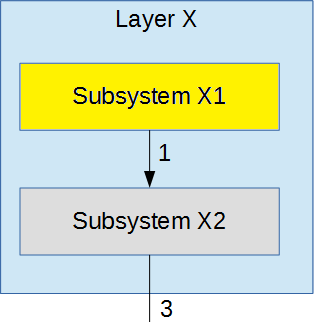
\includegraphics[width=0.60\textwidth]{images/subsystem}
 \caption{Example subsystem description diagram}
\end{figure}

\subsubsection{Assumptions}
The batteries are expected to allow the user to ride the long board for at least 30 minutes without requiring recharging.

\subsubsection{Responsibilities}
The Batteries would ideally provide around 24V which would then be stepped down to 19V for the Jetson TX-2 and 5V if an auxiliary microcontroller is connected.

\subsubsection{Subsystem Interfaces}
Each of the inputs and outputs for the subsystem are defined here.

\begin {table}[H]
\caption {Power Delivery System interfaces} 
\begin{center}
    \begin{tabular}{ | p{1cm} | p{6cm} | p{3cm} | p{3cm} |}
    \hline
    ID & Description & Inputs & Outputs \\ \hline
    \#1 & Power Delivery & \pbox{3cm}{N/A} & \pbox{3cm}{19V/5V}  \\ \hline
    \end{tabular}
\end{center}
\end{table}
